\section{Assignment B16}

\begin{problem}
    The charge, $Q$ coulombs, on the capacitor in an electrical circuit is governed by Kirchhoff's Second Law, which satisfies the differential equation \[L \der[2]{Q}{t} + R \der{Q}{t} + \frac{Q}{C} = V(t),\] where $L$ is the inductance (in henries), $R$ the resistance (in ohms), $C$ the capacitance (in farads) and $V(t)$ is the applied voltage (in volts).

    The initial charge $Q$ and initial current $\derx{Q}{t}$ in a circuit are both zero.

    Given that $L = 0.5$ henries, $R = 10$ ohms, $C = 0.02$ farads and $V(t) = 50\e^{-10t}$, solve for the charge $Q$ at time $t$ and sketch your solution curve.
\end{problem}
\begin{solution}
    Substituting the given values of $L$, $R$, $C$ and $V(t)$, the differential equation becomes \[0.5 \der[2]{Q}{t} + 10 \der{Q}{t} + \frac{Q}{0.02} = 50 \e^{-10t},\] which simplifies as \[\der[2]{Q}{t} + 20 \der{Q}{t} + 100 Q = 100 \e^{-10t}.\] The characteristic equation $r^2 + 20r + 100 = (r+10)^2 = 0$ has the single root $r = -10$. Thus, \[Q_c = \bp{A + Bt} \e^{-10t}.\] For the particular solution, we try \[Q_p = Ct^2 \e^{-10t} \implies \der{Q_p}{t} = C\e^{-10t} \bp{2t - 10t^2} \implies \der[2]{Q_p}{t} = C\e^{-10t} \bp{2 - 40t + 100t^2}.\] Substituting this into the differential equation, we get \[C\e^{-10t} \bp{2 - 40t + 100t^2} + 20C\e^{-10t} \bp{2t - 10t^2} + 100Ct^2 \e^{-10t} = 100\e^{-10t},\] whence $C = 50$ upon simplification. Thus, \[Q = Q_c + Q_p = \bp{A + Bt} \e^{-10t} + 50 t^2 \e^{-10t}.\] Note that \[\der{Q}{t} = \e^{-10t} \bp{B - 10 A - 10B t + 100 t - 500t^2}.\] Since $Q = 0$ and $\derx{Q}{t} = 0$ at $t = 0$, we get $A = 0$ and $B = 10A = 0$. Hence, \[Q = 50 t^2 \e^{-10t}.\]

    \begin{figure}[H]\tikzsetnextfilename{411}
    \centering
    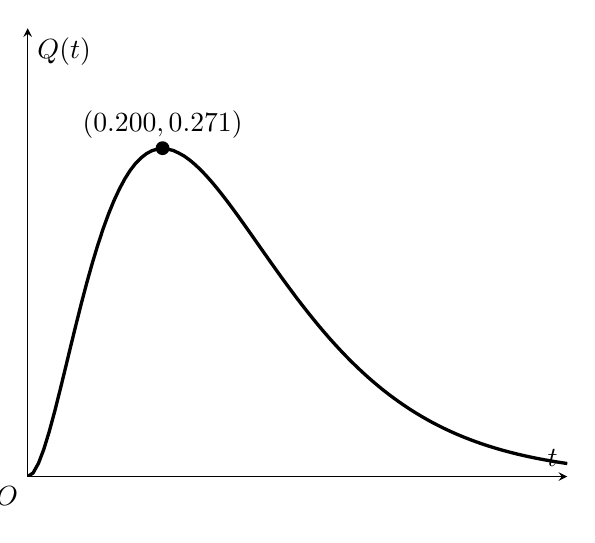
\begin{tikzpicture}[trim axis left, trim axis right]
        \begin{axis}[
            domain = 0:0.8,
            ymin=0,
            ymax=0.37,
            samples = 101,
            axis y line=middle,
            axis x line=middle,
            xtick = \empty,
            ytick = \empty,
            xlabel = {$t$},
            ylabel = {$Q(t)$},
            legend cell align={left},
            legend pos=outer north east,
            after end axis/.code={
                \path (axis cs:0,0) 
                node [anchor=north east] {$O$};
                }
            ]
            \addplot[black, very thick] {50 * x^2 * e^(-10*x)};
            \fill (0.2, 0.271) circle[radius=2.5pt] node[anchor=south] {$(0.200, 0.271)$};
        \end{axis}
    \end{tikzpicture}
    \end{figure}
\end{solution}

\begin{problem}
    Given that $y$ is a function of $x$ and $x = \tan \t$, show that \[\bp{1 + x^2} \der{y}{x} = \der{y}{\t}.\] Hence, show that the differential equation \[\bp{1 + x^2}^3 \der[2]{y}{x} + 2\bp{1 + x^2}^2 \bp{1 + x} \der{y}{x} - 3\bp{1 + x^2} y = x^2 + 6x - 1\] can be expressed as \[\der[2]{y}{\t} + a \der{y}{\t} + by = c \sin 2\t + d \cos 2\t,\] where $a$, $b$, $c$ and $d$ are constants to be determined.

    Hence, find the general solution for $y$ in terms of $x$.
\end{problem}
\begin{solution}
    Note that \[\der{x}{\t} = \sec^2 \t = \tan^2 \t + 1 = x^2 + 1.\] Thus, \[\der{y}{\t} = \der{y}{x} \der{x}{\t} = \bp{1 + x^2} \der{y}{x}.\] Differentiating once more with respect to $\t$, \[\der[2]{y}{\t} = \bp{1 + x^2} \der[2]{y}{x} \der{x}{\t} + 2x \der{x}{\t} \der{y}{x} = \bp{1 + x^2}^2 \der[2]{y}{x} + 2x \der{y}{\t}.\] Dividing the given DE by $1 + x^2$, we have \[\bp{1 + x^2}^2 \der[2]{y}{x} + 2\bp{1 + x^2} \bp{1 + x} \der{y}{x} - 3 y = \frac{x^2 + 6x - 1}{1 + x^2}.\] We can rewrite this as \[\bp{1 + x^2}^2 \der[2]{y}{x} + 2x\der{y}{\t} + 2\der{y}{\t} - 3 y = \frac{x^2 + 6x - 1}{1 + x^2},\] which quickly simplifies as \[\der[2]{y}{\t} + 2 \der{y}{\t} - 3y =  \frac{x^2 + 6x - 1}{1 + x^2}.\] Now, observe that \[\frac{x^2 + 6x - 1}{1 + x^2} = \frac{\tan^2 \t + 6\tan \t - 1}{\sec^2 \t} = \sin^2 \t + 6\sin\t\cos\t - \cos^2\t = 3\sin2\t - \cos2\t.\] Thus, \[\der[2]{y}{\t} + 2 \der{y}{\t} - 3y = 3\sin2\t - \cos2\t,\] whence $a = 2$, $b = -3$, $c = 3$ and $d = -1$.
	
	Note that the characteristic equation $r^2 + 2r - 3 = (r+3)(r-1) = 0$ has roots $r = 1$ and $r = -3$. Thus, \[y_c = A\e^{\t} + B\e^{-3\t}.\] For the particular solution, we try \[y_p = C\sin 2\t + D \cos 2\t.\] Note that \[y_p' = 2C \cos 2\t - 2D \sin 2\t \quad \land \quad y_p'' = -4C \sin 2\t - 4D \cos 2\t.\] Substituting this into the DE, we get
    \begin{gather*}
        \bp{-4C \sin 2\t - 4D \cos 2\t} + 2\bp{2C \cos 2\t - 2D \sin 2\t} - 3\bp{C\sin 2\t + D \cos 2\t}\\
        = 3\sin 2\t - \cos 2\t.
    \end{gather*}
    Comparing coefficients, we get \[\systeme[CD]{-7C-4D = 3,4C-7D=-1},\] whence $C = -5/13$ and $D = -1/13$. Thus, \[y = y_c + y_p =  A\e^{\t} + B\e^{-3\t} - \frac5{13} \sin 2\t - \frac1{13} \cos 2\t.\] Substituting $\t = \arctan x$, \[y = A\e^{\arctan x} + B\e^{-3\arctan x} - \frac5{13} \sin{2\arctan x} - \frac1{13} \cos{2\arctan x}.\]
\end{solution}

\begin{problem}
    An object of mass $m$, in kilograms, is suspended from one end of a vertical spring of elasticity $k$, $k > 0$, in a resistive medium with resistivity $c$, $c > 0$. When the object is pulled down from its equilibrium position and released, the motion of the object can be described by the following differential equation, where $y$ is the displacement, in metres, of the object from the equilibrium position after time $t$. \[\der[2]{y}{t} + \frac{c}{m} \der{y}{t} + \frac{k}{m} y = 0.\]

    \begin{enumerate}
        \item The diagram below shows how $y$ varies with $t$ for some values of $c$, $m$ and $k$.
        \begin{figure}[H]\tikzsetnextfilename{412}
        \centering
        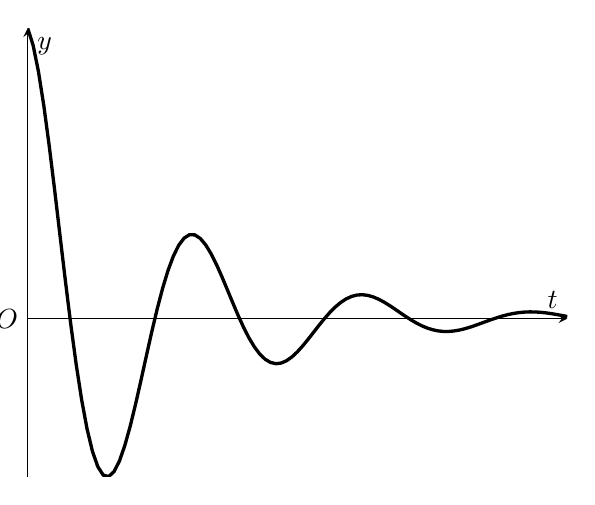
\begin{tikzpicture}[trim axis left, trim axis right]
            \begin{axis}[
                domain = 0:20,
                restrict y to domain =-4:8,
                samples = 101,
                axis y line=middle,
                axis x line=middle,
                xtick = \empty,
                ytick = \empty,
                xlabel = {$t$},
                ylabel = {$y$},
                legend cell align={left},
                legend pos=outer north east,
                after end axis/.code={
                    \path (axis cs:0,0) 
                    node [anchor=east] {$O$};
                    }
                ]
                \addplot[black, very thick] {6 * cos(\x r) * e^(-0.2*x)};
            \end{axis}
        \end{tikzpicture}
        \end{figure}
        State the condition(s) for $c$, $m$ and $k$ for the above scenario.
    \end{enumerate}

    When an external force, $F(t)$, is applied to the object, the motion of the object can be described by the following modified differential equation: \[\der[2]{y}{t} + \frac{c}{m} \der{y}{t} + \frac{k}{m} y = F(t).\]

    \begin{enumerate}
        \setcounter{enumi}{1}
        \item For the same $c$, $m$ and $k$ in part (a), sketch a graph of $y$ versus $t$ for
        \begin{enumerate}
            \item $F(t) = a$,
            \item $F(t) = b\e^{-t}$,
        \end{enumerate}
        where $a$ and $b$ are positive constants, showing the long-term behaviour of $y$.
        \item In another setup, the resistivity is approximately equal to 0, that is $c = 0$. Given that the external force is $F(t) = \sin wt$, where $w^2 = k/m$, the differential equation is now \[\der[2]{y}{t} + w^2 y = \sin wt.\] Solve for $y$, in terms of $w$ and $t$, if the object is initially at the equilibrium position with zero velocity.
    \end{enumerate}
\end{problem}
\begin{solution}
    \begin{ppart}
        Note that the characteristic equation of the DE is given by \[r^2 + \frac{c}{m} r + \frac{k}{m} = 0 \implies m r^2 + cr + k = 0.\] For $y$ to oscillate (i.e. composed of sine and cosine terms), the roots of the characteristic equation must be non-real. We hence obtain the constraint \[\D = c^2 - 4mk < 0.\]
    \end{ppart}
    \begin{ppart}
        Note that the given graph represents the complementary solution.
        \begin{psubpart}
            Let the particular solution be a constant $z$. Substituting this into the DE, we get $kz/m = a$, whence $z = am/k$, which is a positive constant. Hence, we simply shift the graph of $y(t)$ in the positive $y$-axis.

            \begin{figure}[H]\tikzsetnextfilename{413}
                \centering
                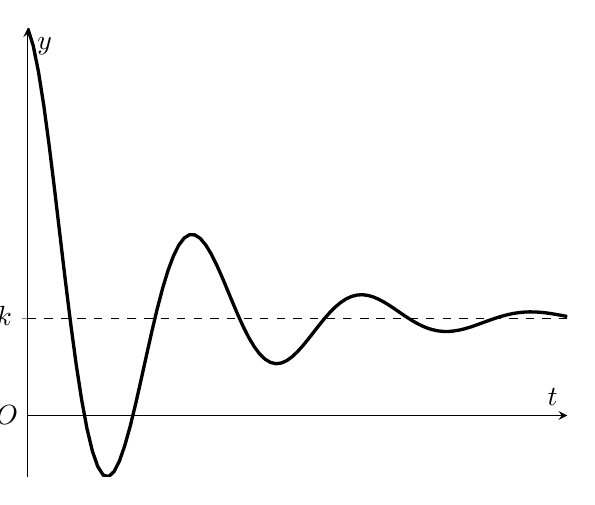
\begin{tikzpicture}[trim axis left, trim axis right]
                    \begin{axis}[
                        domain = 0:20,
                        restrict y to domain =-4:8,
                        samples = 101,
                        axis y line=middle,
                        axis x line=middle,
                        xtick = \empty,
                        ytick = {2},
                        yticklabels = {$am/k$},
                        xlabel = {$t$},
                        ylabel = {$y$},
                        legend cell align={left},
                        legend pos=outer north east,
                        after end axis/.code={
                            \path (axis cs:0,0) 
                            node [anchor=east] {$O$};
                            }
                        ]
                        \addplot[black, very thick] {6 * cos(\x r) * e^(-0.2*x) + 2};
                        \addplot[dashed] {2};
                    \end{axis}
                \end{tikzpicture}
            \end{figure}
        \end{psubpart}
        \clearpage
        \begin{psubpart}
            Since $F(t) = b\e^{-t}$, the particular solution is of the form $C\e^{-t}$. The resulting graph hence oscillates around $C\e^{-t}$:

            \begin{figure}[H]\tikzsetnextfilename{414}
                \centering
                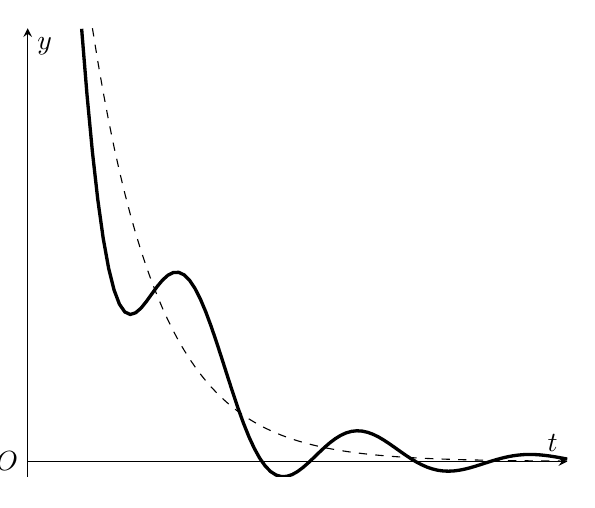
\begin{tikzpicture}[trim axis left, trim axis right]
                    \begin{axis}[
                        domain = 0:20,
                        restrict y to domain =-1:10,
                        samples = 101,
                        xmin=0,
                        axis y line=middle,
                        axis x line=middle,
                        xtick = \empty,
                        ytick = \empty,
                        xlabel = {$t$},
                        ylabel = {$y$},
                        legend cell align={left},
                        legend pos=outer north east,
                        after end axis/.code={
                            \path (axis cs:0,0) 
                            node [anchor=east] {$O$};
                            }
                        ]
                        \addplot[black, very thick] {6 * cos(\x r) * e^(-0.2*x) + 25 * e^(-0.4*x)};
                        \addplot[dashed] {25 * e^(-0.4*x)};
                    \end{axis}
                \end{tikzpicture}
            \end{figure}
        \end{psubpart}
    \end{ppart}
    \begin{ppart}
        Note that the characteristic equation is $r^2 + r^2 = 0$, whence $r = \pm \i w$. Thus, \[y_c = A\cos wt + B\sin wt.\] For the particular solution, we try \[y_p = Ct\sin wt + Dt \cos wt.\] Note that \[y_p' = wt \bp{C\cos wt - D \sin wt} + C\sin wt + D \cos wt\] and \[y_p'' = w^2 t \bp{-C\sin wt - D \cos wt} + 2w \bp{C \cos wt - D \sin wt}.\] Substituting this into the DE, we get
        \begin{gather*}
            w^2 t \bp{-C\sin wt - D \cos wt} + 2w \bp{C \cos wt - D \sin wt} \\
            + w^2 \bp{Ct\sin wt + Dt \cos wt} = \sin wt.
        \end{gather*}
        Comparing coefficients, we obtain $C = 0$ and $D = -1/2w$. Thus, \[y = y_c + y_p = A\cos wt + B \sin wt - \frac{t}{2w} \cos wt.\] Note that \[y' = -Aw \sin wt + Bw \cos wt - \frac1{2w} \bp{\cos wt - tw\sin wt}.\] Since $y(0) = y'(0) = 0$, we have $A = 0$ and \[Bw - \frac1{2w} = 0 \implies B = \frac1{2w^2}.\] Thus, \[y = \frac1{2w^2} \sin wt - \frac{t}{2w} \cos wt.\]
    \end{ppart}
\end{solution}